\section{Компьютерная морфология}\label{sect_review_comp_morphology}

Морфология -- это раздел лингвистики, изучающий структуру слова и его грамматические значения~\cite{MitreninaNikolaevLando2016}. Другими словами, морфология изучает
1) часть речи,
2) словоизменение,
3) словообразование,
4) грамматическое значение (что слово означает в предложении).

Компьютерная морфология анализирует и синтезирует слова программными средствами~\cite{MitreninaNikolaevLando2016}.

В компьютерной морфологии взаимосвязаны три базовых понятия: лемма, граммема и словоформа.
\begin{enumerate}
    \item \emph{Лемма}~-- это базовая, каноническая форма слова.
        Например, инфинитив у глагола.

    \item Грамматическое значение представляется в виде набора \emph{граммем}.
        Граммему также называют грамматической характеристикой,
          морфологическим признаком, морфологическим свойством,
          тегом (при разметке текста).
        Граммемы группируются по категориям (падеж, время и т.~д.).
        Одна и та же форма слова не может иметь две граммемы одной категории
        (например, глагол не может иметь сразу форму прошлого и настоящего времени).
        С другой стороны, формы могут совпадать, и их нужно уметь различать.

    \item \emph{Словоформа}~-- это\ldots \TODO{TODO}
\end{enumerate}

\bigskip 
\TODO{TODO: Добавить определения и пояснения (здесь лексема и парадигма, в след. раздел --- лемматизация) см. http://macrocosm.narod.ru/lingvo.html}
\bigskip 

\emph{Лингвистическа разметка}~--- это процесс или результат 
приписывания текстам и их компонентам специальных меток, 
позволяющих выполнять поиск по лингвистическому корпусу~\cite[415]{Kibrik2019}.
%
В корпусной лингвистике есть ряд требований к разметке, известных как 
семь максим Лича~\cite[415--416]{Kibrik2019}. 


\subsubsection{Морфологическое словоизменение и морфологический анализ}

Морфологическое словоизменение\footnote{%
    \emph{Морфологическое словоизменение} по-английски звучит как
    ``inflectional morphology''.
    \emph{Система} и \emph{задача морфологического словоизменения}
    будут переводиться как
    ``morphological inflection system'' и ``morphological inflection task'' соответственно,
    см. например, американскую статью~\cite{King2020seq2seqRussianMA}.
} или просто словоизменение~--
это отображение лемм и набора морфологических признаков
на соответствующую словоформу~\cite[2821]{Cruz-Anastasopoulos-Stump2020Chatino}.

Под \emph{морфологическим анализом} слова или словоформы (morphological analysis)
подразумевается определение леммы и
грамматических характеристик словоформы~\cite{MitreninaNikolaevLando2016}.

Таким образом, если задачу <<морфологического словоизменения>> обозначить как прямую
(по лемме и признаку нужно найти словоформу),
то <<морфологический анализ>> (по словоформе требуется найти
лемму и морфологические свойства) будет обратной задачей (рис.~\ref{fig:inflectional_operations}).

\begin{figure}
    \centering
    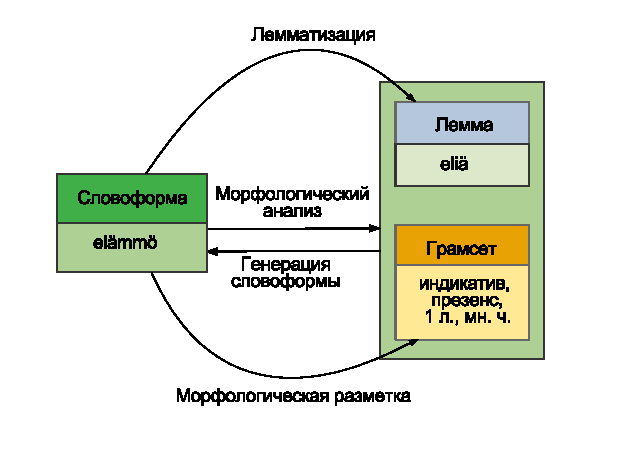
\includegraphics[width=0.75\textwidth,keepaspectratio=true]{inflectional_operations_v2}
%      \includegraphics[width=1\linewidth]{inflectional_operations.pdf}
    \caption[Четыре морфологические операции: генерация, анализ, лемматизация и разметка]{Четыре 
        морфологические операции: генерация, анализ, лемматизация и разметка 
        на примере карельского глагола ``eliä''\footnotemark.  
        Лемма ``eliä'' (жить), словоформа ``elämmö'' (живём). 
        Адаптация рисунка из статьи~\cite{Nicolai2020FineGraned}.} 
    \label{fig:inflectional_operations}
\end{figure}

Отметим, что в ряде языков отсутствует морфологическое словоизменение,
например, в языках йоруба и севернокитайском~\cite[2]{Vylomova2020SIGMORPHON}.

\footnotetext{См. словарную статью ``eliä'' на сайте корпуса ВепКар \url{http://dictorpus.krc.karelia.ru/ru/dict/lemma/4651}.}


\subsubsection{Paradigm Cell Filling Problem}

С задачей морфологического анализа тесно связана задача
``a paradigm cell filling problem'' (PCFP)~\cite{Ackerman08PartsAndWholes}.



\subsubsection{Соревнования по морфологическому анализу (и результаты?)}

Рассмотренные выше задачи решают на соревнованиях
между компьютерными программами в рамках различных конференций:
\begin{description}[align=left]
    \item [Диалог]\footnote{См. \url{http://www.dialog-21.ru}}~--
            известная отечественная конференция
            по компьютерной лингвистике.
            В 2019 году в преддверии этой конференции
            было проведено соревнование LowResourceEval
            по анализу нескольких языков России~\cite{Klyachko2019LowresourceEval}.
        \TODO{TODO коротенько о главных результатах.}

    \item [SIGMORPHON]\label{SIGMORPHON}\footnote{См. \url{https://sigmorphon.github.io}}~--
                это группа учёных (одна из множества групп ACL\footnote{%
                ACL расшифровывается как ``Association for Computational Linguistics''.
                Ассоциация компьютерной лингвистики~-- это
                международное научное и техническое сообщество специалистов
                по обработке текстов и языковой информации.
            }),
            занимающихся вычислительной морфологией и фонологией,
            и одноимённая конференция, проводимая этими учёными.
            В соревновании по морфологии ``SIGMORPHON 2020''
            были использованы данные
            разрабатываемого корпуса ВепКар~\cite{Vylomova2020SIGMORPHON}.

            \TODO{TODO коротенько о главных результатах.}
\end{description}



\subsection{Малоресурсные языки}\label{sect_low-resource}

Языки, которым посвящена эта работа, то есть вепсский и карельский,
относят к малоресурсным языкам~\TODO{TODO: доказательная ссылка}.

Есть интуитивное представление, что \emph{малоресурсные языки}~---
это языки, обладающие недостаточным объёмом текстов
в бумажном и электронном виде,
имеющие слабую компьютерную поддержку.
То есть для таких языков может не быть
электронных словарей, лингвистических корпусов,
систем проверки правописания, систем машинного перевода,
либо они есть, но несопоставимы по качеству и объёму с теми же объектами
высокоресурсных языков.
\TODO{TODO: сделать таблицу с рядом языков России
и наличием таких ресурсов у них. И решением
о мало-, высокоресурсности языков.}.

\TODO{Термин «малоресурсные языки» (under-resourced languages или low-resourced languages) первоначально был предложен нидерландским ученым С. Краувером [Krauwer S. The basic language resource kit (BLARK) as the first milestone for the language resources roadmap. In Proc. International Workshop on Speech and Computer SPECOM-2003. Moscow, Russia, pp. 8-15, 2003]. Это понятие относится к естественным языкам с некоторыми (или всеми) из следующих свойств: недостаток своей системы письменности или устойчивой орфографии; нехватка квалифицированных лингвистов и переводчиков для данного языка; ограниченное распространение в сети Интернет; нехватка электронных ресурсов для обработки языка и речи, в том числе одноязычных корпусов, двуязычных электронных словарей, орфографических и фонетических транскрипций речи, словарей произношения, автоматических технологий обработки языка и речи и т. д.}

В работе~\cite{Anastasopoulos2019Pushing_Limits_Low-Resource_MI}
предложены численные границы для малоресурсных и высокоресурсных языков. 
Малоресурсные языки содержат около 100 примеров в обучающем наборе
и 50-100 (редко 1000) примеров в настраивающем наборе данных\footnote{%
    В машинном обучении обычно выделяют три типа
    последовательно используемых данных: training, validation и test sets.
    \begin{enumerate}[label=(\roman*)]
        \item \emph{training set} (тестовый набор данных)~--
            это набор данных для настройки весов, например, матрицы,
            где эти веса вычисляются с помощью нейронных сетей.

        \item \emph{validation set, development set, dev set}
            (настраивающий или настроечный набор данных)~--
            набор данных для настройки гиперпараметров нейронной сети,
            например, число нейронов в каждом слое.

        \item \emph{test set} (тестовый набор данных)~-- это набор данных
            для оценки полученной модели.
    \end{enumerate}
    }% eo footnote
%
.
Большинство высокоресурсных языков содержат по 10\,000 примеров.
Эти цифры приводятся на примере данных,
предоставленных участникам соревнования SIGMORPHON 2019 года\footnote{%
    См. о SIGMORPHON на с.~\pageref{SIGMORPHON}.
    Данные соревнования ``SIGMORPHON 2020 task 0'', представленные
    в таблице \TODO{(TODO ссылка на таблицу)},
    доступны по
    ссылке~\url{https://github.com/sigmorphon2020/task0-data}.
}~\cite{Anastasopoulos2019Pushing_Limits_Low-Resource_MI}.


\TODO{Перевести данные в табличку с размерами train, dev и test set для языков 
ВепКар на SIGMORPHON 2020
И на основе этого сделать вывод, какие из наших языков мало- или много- 
ресурсные.}

SIGMORPHON 2020 task 0

vep  train 94\,395 dev 13\,320 test 26\,422

krl  train 80\,216 dev 11\,225 test 22\,290

olo  train 43\,936 dev 6\,260 test 12\,515

lud  train 294 dev 41 test 82

\begin{table}
%\begin{adjustbox}{width=1\textwidth}
\small
\centering
\small
\begin{tabular}{c|r|r|r|r|r|r|>{\hspace{2em}}r|r|>{\hspace{2em}}r|r}
\toprule
%\multicolumn{1}{c}{\textbf{Lang}}&\multicolumn{3}{c}{\textbf{Total}}\\
\textbf{Язык / Наречие} & \textbf{Код языка} & \textbf{Train} & \textbf{Dev} & \textbf{Test} \\
%\cmidrule(lr){1-1} \cmidrule(lr){2-4} \cmidrule(lr){5-7} \cmidrule(lr){8-9} \cmidrule(lr){10-11}
% &Train& Dev & Test \\

\midrule
Карельский: собственно карельское наречие & krl&80216&11225&22290\\
Карельский: людиковское наречие & lud&294&41&82\\
Карельский: ливвиковское наречие & olo&43936&6260&12515\\
Вепсский & vep&94395&13320&26422\\
%\midrule
%est&26728&3820&7637&2.7&0.4&0.8&6.1&5.1&22.4&11.6\\
%fin&99403&14201&28401&0.0&0.0&0.0&0.0&0.0&32.6&17.2\\
%izh&763&112&224&0.0&0.0&0.0&0.0&0.0&42.9&22.3\\
%liv&2787&398&802&0.0&0.0&0.0&0.0&0.0&40.7&24.1\\
%\midrule
%ang&29270&4122&8197&11.8&1.8&3.4&21.6&21.9&35.1&21.3\\
%aze&5602&801&1601&11.9&1.9&4.0&22.3&20.9&31.5&20.2\\
%cre&4571&584&1174&18.5&2.1&4.9&29.8&29.6&5.5&2.7\\
%dan&17852&2550&5101&16.5&2.5&5.0&34.5&32.9&71.4&51.8\\
%nob&13263&1929&3830&10.5&1.8&3.1&18.5&19.7&80.5&70.5\\
%pei&10017&1349&2636&15.8&2.6&4.9&21.5&21.4&9.1&4.7\\
\bottomrule
\end{tabular}
%\end{adjustbox}
\caption{Number of samples in training, development, test sets, as well as statistics on systematic errors (inconsistency) and percentage of samples with lemmata observed in the training set.
(VepKar languages, other Uralic languaes and languages with the highest rates of inconsistency, see~\cite{Vylomova2020SIGMORPHON})
}
\label{tab:lang-stats}
\end{table}

\newpage\clearpage


\begin{tabular}{llr}
\hline
\multicolumn{2}{c}{Item} \\
\cline{1-2}
Animal    & Description & Price (\$) \\
\hline
Gnat      & per gram    & 13.65      \\
          & each        & 0.01       \\
Gnu       & stuffed     & 92.50      \\
Emu       & stuffed     & 33.33      \\
Armadillo & frozen      & 8.99       \\
\hline
\end{tabular}



\bigskip
\bigskip





\subsection{Обзор компьютерных программ для морфологической обработки}

\subsection{Финский язык}\label{sect_review_fin}

Статья о лемматизаторе FinnPos~\cite{silfverberg2016finnpos}.

%https://github.com/mpsilfve/FinnPos


\bigskip
\bigskip
